\documentclass[handout]{beamer}
%\documentclass [serif,mathserif,professionalfont]{beamer} 
%\usepackage {pxfonts}
%\usepackage {eulervm}
%\usepackage{mathpazo}
%\logo{\includegraphics[height=1.2cm]{fsulogo.png}}
\usepackage{amsmath,amsthm,verbatim,amssymb,amsfonts,amscd,color,graphicx}
\usepackage{graphics,tikz,pgflibraryarrows,pgflibrarysnakes,booktabs,multirow,color}
\usepackage{hyperref,setspace}

\usepackage{tikz}
\usepackage{graphicx}
\usepackage{multimedia}
\usepackage[latin1]{inputenc}
%\usetheme{Warsaw}
\usecolortheme{lily}
\setbeamercovered{transparent}
%\useoutertheme[subsection=false]{smoothbars}


\setbeamertemplate{navigation symbols}
{Population Histroy Estimation: A Coalescent Theory Approach
~
\insertslidenavigationsymbol
%\insertsubsectionnavigationsymbol  
% \insertsectionnavigationsymbol
% \insertdocnavigationsymbol  
%\insertbackfindforwardnavigationsymbol 
\hspace{1em}  
\usebeamerfont{footline} 
%\setbeamercolor{footline}{fg=blue}
\insertframenumber/\inserttotalframenumber }
\setcounter{page}{1} 
\pagenumbering{arabic} 

\title{Population History Estimations: \\ A Coalescent Theory Approach}
%[EVA, Ann Arbor, MI 2015 \insertdate]
\author{Xuehua \textsc{Lan}\\ \textit{Supervisor: \small{Nathan \textsc{Ross}}}}
\institute{The University of Melbourne \\  Deaprtment of Mathematics and Statistics}
\date{May, 2017}

\begin{document}
\pagenumbering{arabic}
\begin{frame}
\titlepage
\end{frame}


\begin{frame}{Human Migration out of Africa}
\begin{center}
\includegraphics[scale=0.5]{Africa.png}
\end{center}
\footnotesize{Source~$https://wikimedia.org/wiki/File:Human$\underline{~}$migration$\underline{~}$out$\underline{~}$of$\underline{~}$Africa$}
\end{frame}
%------------------------------------------
%------------------------------------------
\begin{frame}{Interest: is there a bottleneck?}
\begin{figure}
\begin{center}
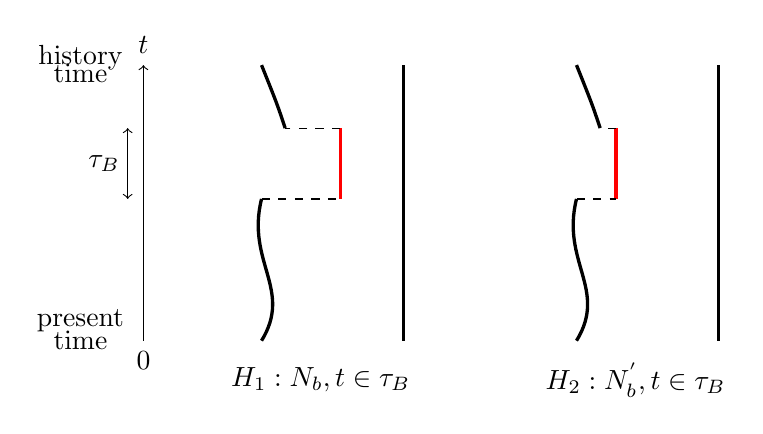
\begin{tikzpicture}%[thick,scale=0.7, every node/.style={scale=0.7}]
\draw [->] (-4.5,1)--(-4.5,4.5);
\node at (-4.5,4.75) {$t$};
\node at (-4.5,0.75) {$0$};
\draw [line width=1.2] (-3,1)..controls (-2.6,1.65) and (-3.2,2).. (-3,2.8);
\draw [line width=1.2] [red](-2,2.8)--(-2,3.7);
\draw [line width=1.2] (-2.7,3.7)..controls (-2.8,4).. (-3,4.5);
\draw [dashed] (-3,2.8)--(-2,2.8);
\draw [dashed] (-2,3.7)--(-2.7,3.7);
\draw [line width=1.2] (-1.2,1)--(-1.2,4.5);
\draw [line width=1.2] (1,1)..controls (1.4,1.65) and (0.8,2).. (1,2.8);
\draw [line width=1.2] [red](1.5,2.8)--(1.5,3.7);
\draw [line width=1.2] (1.3,3.7)..controls (1.2,4).. (1,4.5);
\draw [dashed] (1,2.8)--(1.5,2.8);
\draw [dashed] (1.5,3.7)--(1.3,3.7);
\draw [line width=1.2] (2.8,1)-- (2.8,4.5);
\node at (-2.25,.5) {$H_{1}:N_{b}, t\in\tau_{B}$};
\node at (1.75,.5) {$H_{2}:N_{b}^{'}, t\in\tau_{B}$};
\draw [<->] (-4.7,2.8)--(-4.7,3.7);
\node at (-5,3.25) {$\tau_{B}$};
\node at (-5.3,1.25) {present};
\node at (-5.3,1) {time};
\node at (-5.3,4.6) {history};
\node at (-5.3,4.4) {time};
\end{tikzpicture}
\end{center}
\end{figure}
\end{frame}
%------------------------------------------
\begin{frame}{Interest: when is the diverging time?}
\begin{figure}
\begin{center}
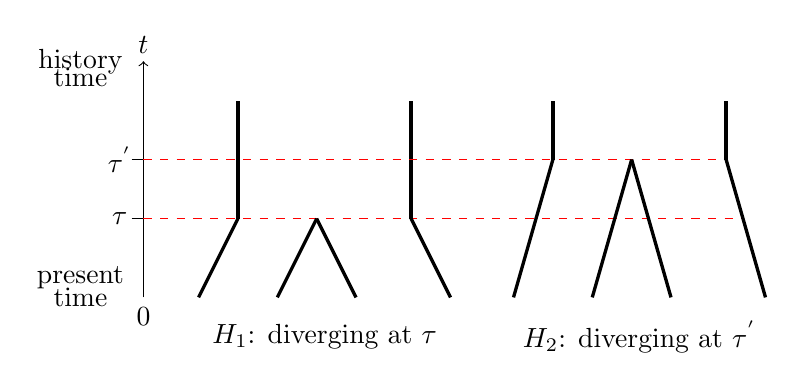
\begin{tikzpicture}%[thick,scale=0.6, every node/.style={scale=0.6}]
\draw[->] (0.3,0) --(0.3,3);
\node at (0.3, -0.25) {$0$};
\node at (0.3, 3.2) {$t$};
\node at (-0.5,0.25) {present};
\node at (-0.5,0) {time};
\node at (-0.5,3) {history};
\node at (-0.5,2.8) {time};
%population 1
\draw (0.15,1) -- (0.3,1);
\node at (0,1) {$\tau$};
\draw [red][dashed] (0.3,1)--(7.9,1);
\draw [line width=1.2](1.5,1)--(1.5,2.5);
\draw [line width=1.2](3.7,1)--(3.7,2.5);
\draw [line width=1.2](1,0)--(1.5,1);
\draw [line width=1.2](4.2,0)--(3.7,1);
\draw [line width=1.2](2,0)--(2.5,1);
\draw [line width=1.2](3,0)--(2.5,1);
\node at (2.6,-.5) {$H_{1}$: diverging at $\tau$};
%population 2
\draw (0.15,1.75) -- (0.3,1.75);
\node at (0,1.75) {$\tau^{'}$};
\draw [red][dashed] (0.3,1.75)--(7.7,1.75);
\draw [line width=1.2](5.5,1.75)--(5.5,2.5);
\draw [line width=1.2](7.7,1.75)--(7.7,2.5);
\draw [line width=1.2](5,0)--(5.5,1.75);
\draw [line width=1.2](8.2,0)--(7.7,1.75);
\draw [line width=1.2](6,0)--(6.5,1.75);
\draw [line width=1.2](7,0)--(6.5,1.75);
%notes
\node at (6.6,-.5) {$H_{2}$: diverging at $\tau^{'}$};
\end{tikzpicture}
\end{center}
\end{figure}
\end{frame}
%\section{Introduction}

%------------------------------------------
\begin{frame}{Introduction}
\begin{block}{Interests}
theoretical lower bounds w.r.t. amount of data used.
\end{block}
\begin{block}{Outlines}
\begin{itemize}
  \item Models
  \item Statistics
  \item Data used
  \item Lower Bounds
  \item Results
\end{itemize}
\end{block}
\end{frame}
%--------------------------------------------
\begin{frame}{Wright-Fisher Model and Coalescent}
\begin{itemize}
\item Wright-Fisher: population has constant size N\\ ${~~~~~~~~~~~~~~~~~~~}$uniformly sampling for parents
\item Coalescent: find the most recent common ancestor (MRCA)
\end{itemize}
\begin{figure}
\begin{center}
\tikzstyle{rplace}=[circle,fill=red!75,thick]
\tikzstyle{gplace}=[circle,fill=blue!75,thick]
\tikzstyle{wplace}=[circle,draw=black!100,thick]
\begin{tikzpicture}[thick,scale=0.8, every node/.style={scale=0.8}]
\node at (1,6) [rplace] {};
\node at (2,6) [wplace] {};
\node at (3,6) [wplace] {};
\node at (4,6) [wplace] {};
\node at (5,6) [wplace] {};
\node at (6,6) [gplace] {};
\node at (1,5) [wplace] {};
\node at (2,5) [rplace] {};
\node at (3,5) [wplace] {};
\node at (4,5) [wplace] {};
\node at (5,5) [wplace] {};
\node at (6,5) [gplace] {};
\node at (1,4) [wplace] {};
\node at (2,4) [rplace] {};
\node at (3,4) [wplace] {};
\node at (4,4) [wplace] {};
\node at (5,4) [gplace] {};
\node at (6,4) [gplace] {};
\node at (1,3) [rplace] {};
\node at (2,3) [wplace] {};
\node at (3,3) [wplace] {};
\node at (4,3) [gplace] {};
\node at (5,3) [gplace] {};
\node at (6,3) [gplace] {};
\node at (1,2) [rplace] {};
\node at (2,2) [wplace] {};
\node at (3,2) [gplace] {};
\node at (4,2) [gplace] {};
\node at (5,2) [gplace] {};
\node at (6,2) [gplace] {};
\node at (1,1) [rplace] {};
\node at (2,1) [rplace] {};
\node at (3,1) [gplace] {};
\node at (4,1) [gplace] {};
\node at (5,1) [gplace] {};
\node at (6,1) [gplace] {};
\node at (0,6.5) {generation};
\node at (0,6) {$t-5$};
\node at (0,5) {$t-4$};
\node at (0,4) {$t-3$};
\node at (0,3) {$t-2$};
\node at (0,2) {$t-1$};
\node at (0,1) {$t$};
\draw (1,5.8)--(1,5.2);
\draw (1,4.8)--(1,4.2);
\draw (1,5.8)--(2,5.2);
\draw (1,5.8)--(3,5.2);
\draw (2,4.8)--(2,4.2);
\draw (2,3.8)--(1,3.2);
\draw (2,3.8)--(2,3.2);
\draw (1,2.8)--(1,2.2);
\draw (1,2.8)--(2,2.2);
\draw (1,1.8)--(1,1.2);
\draw (1,1.8)--(2,1.2);
\draw (5,5.8)--(4,5.2);
\draw (4,4.8)--(3,4.2);
\draw (4,4.8)--(4,4.2);
\draw (3,3.8)--(3,3.2);
\draw (6,5.8)--(5,5.2);
\draw (6,5.8)--(6,5.2);
\draw (6,4.8)--(5,4.2);
\draw (6,4.8)--(6,4.2);
\draw (5,3.8)--(4,3.2);
\draw (6,3.8)--(5,3.2);
\draw (6,3.8)--(6,3.2);
\draw (4,2.8)--(3,2.2);
\draw (5,2.8)--(4,2.2);
\draw (5,2.8)--(5,2.2);
\draw (6,2.8)--(6,2.2);
\draw (3,1.8)--(3,1.2);
\draw (4,1.8)--(4,1.2);
\draw (5,1.8)--(5,1.2);
\draw (6,1.8)--(6,1.2);
\node at (6.85,5) {MRCA};
\draw [->](7.7,1)--(7.7,5.8);
\node at (7.7,6.5) {Backward};
\node at (7.7,6.15) {in time};
\end{tikzpicture}
\end{center}
\end{figure}
\end{frame}
%--------------------------------------------
\begin{frame}{Gene Genealogies and Coalescent Tree}
\begin{figure}
\begin{center}
\tikzstyle{rplace}=[circle,fill=red!75,thick]
\tikzstyle{gplace}=[circle,fill=blue!75,thick]
\tikzstyle{bplace}=[circle,fill=green!75,thick]
\tikzstyle{wplace}=[circle,draw=black!100,thick]
\begin{tikzpicture}[thick,scale=0.8, every node/.style={scale=0.8}]
\node at (6,6) [gplace] {};
\node at (5,5) [wplace] {};
\node at (6,5) [gplace] {};
\node at (5,4) [gplace] {};
\node at (6,4) [gplace] {};
\node at (4,3) [gplace] {};
\node at (5,3) [gplace] {};
\node at (6,3) [gplace] {};
\node at (3,2) [gplace] {};
\node at (4,2) [gplace] {};
\node at (5,2) [gplace] {};
\node at (6,2) [gplace] {};
\node at (3,1) [gplace] {};
\node at (4,1) [gplace] {};
\node at (5,1) [gplace] {};
\node at (6,1) [gplace] {};
\node at (2,6.5) {generation};
\node at (2,6) {$t-5$};
\node at (2,5) {$t-4$};
\node at (2,4) {$t-3$};
\node at (2,3) {$t-2$};
\node at (2,2) {$t-1$};
\node at (2,1) {$t$};
\draw (6,5.8)--(5,5.2);
\draw (6,5.8)--(6,5.2);
\draw (6,4.8)--(5,4.2);
\draw (6,4.8)--(6,4.2);
\draw (5,3.8)--(4,3.2);
\draw (6,3.8)--(5,3.2);
\draw (6,3.8)--(6,3.2);
\draw (4,2.8)--(3,2.2);
\draw [red](5,2.8)--(4,2.2);
\draw [red](5,2.8)--(5,2.2);
\draw (6,2.8)--(6,2.2);
\draw (3,1.8)--(3,1.2);
\draw [red](4,1.8)--(4,1.2);
\draw [red](5,1.8)--(5,1.2);
\draw (6,1.8)--(6,1.2);
\node at (6.75,5) {MRCA};
\draw [->](7.7,1)--(7.7,5.8);
\node at (7.7,6.5) {Backward};
\node at (7.7,6.15) {in time};
\draw [line width=1.2](8.5,1)--(8.5,5);
\draw [red][line width=1.2](9.5,1)--(9.5,3);
\draw [red][line width=1.2](10.5,1)--(10.5,3);
\draw [line width=1.2](11.5,1)--(11.5,4);
\draw [red][line width=1.2](9.5,3)--(10.5,3);
\node at (10,3) {$\bullet$};
\draw [line width=1.2](10,3)--(10,4);
\draw [line width=1.2](10,4)--(11.5,4);
\draw [line width=1.2](10.75,4)--(10.75,5);
\draw [line width=1.2](8.5,5)--(10.75,5);
\draw [line width=1.2](9.6325,5)--(9.6325,6.5);
\end{tikzpicture}
\end{center}
\end{figure}
\end{frame}
%--------------------------------------------
\begin{frame}{Kingman Coalescent from Wright-Fisher Model}
\begin{itemize}
\item $n$ sample chosen from population $N$
\end{itemize}
\begin{block}{discrete-time coalescent}
\begin{itemize}
\item 0 coal: $p_{\textcolor{red}{n,n}}=\frac{N-1}{N}\ldots\frac{N-n+1}{N}=\textcolor{red}{1-\frac{n(n-1)}{2N}}+\mathcal{O}(N^{-2})$
\item 1 coal: $p_{\textcolor{red}{n,n-1}}=\frac{N-1}{N}\ldots\frac{N-n+2}{N}\cdot \frac{n(n-1)}{2N}=\textcolor{red}{\frac{n(n-1)}{2N}}+\mathcal{O}(N^{-2})$
\end{itemize}
\end{block}
\begin{block}{continuous-time coalescent}
\begin{itemize}
\item time measured in units of \textcolor{red}{$N$} generations, $N\rightarrow\infty$
\item $t_{\textcolor{red}{n}}$: time for \textcolor{red}{$n$} lineages coalescent into \textcolor{red}{$n-1$} lineages
\begin{align}P(t_{n}>t)=(1-\frac{n(n-1)}{2N})^{N\cdot t}\rightarrow\exp(-t\frac{n(n-1)}{2})\end{align}
\end{itemize}
\end{block}
\end{frame}
%--------------------------------------------
\begin{frame}{Kingman Coalescent with Constant Populations}
\begin{itemize}
\item $n=5$ sample from population $N$
\item time measured in units of $N$ generations
\end{itemize}
\begin{figure}
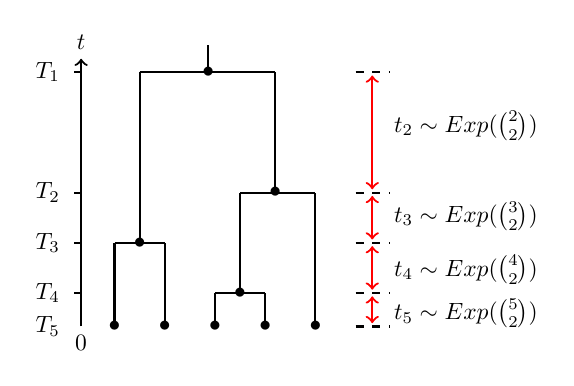
\begin{tikzpicture}[thick,scale=0.85, every node/.style={scale=0.85}]
%picture
%\draw (0,0) node[below]{$~$}--(0,3.8);
%\node at (0,4.25) {lineages};
%\node at (0,3.8) {$\bullet$};
%\node at (0,2) {$\bullet$};
%\node at (0,1.25) {$\bullet$};
%\node at (0,0.5) {$\bullet$};
%\node at (0,0) {$\bullet$};
%\node at (-0.5,0) {$5$};
%\node at (-0.5,0.5) {$4$};
%\node at (-0.5,1.25) {$3$};
%\node at (-0.5,2) {$2$};
%\node at (-0.5,3.8) {$1$};
%\node at (1,-0.75) {$(a)$ Pure Death Process};
%\draw [red][->] (0.5,0.05)--(0.5,0.45);
%\draw [red][->] (0.5,0.55)--(0.5,1.2);
%\draw [red][->] (0.5,1.3)--(0.5,1.95);
%\draw [red][->] (0.5,2.05)--(0.5,3.75);
%\node at (1.5,0.2) {$\mu_{54}=\binom{5}{2}$};
%\node at (1.5,0.85) {$\mu_{43}=\binom{4}{2}$};
%\node at (1.5,1.65) {$\mu_{32}=\binom{3}{2}$};
%\node at (1.5,3) {$\mu_{21}=\binom{2}{2}$};
%picture
\draw[->] (4,0) node[below]{$0$}--(4,4) node[above]{$t$};
\draw (4.5,0)--(4.5,1.25);
\draw (5.25,0)--(5.25,1.25);
\draw (4.875,1.25)--(4.875,3.8);
\draw (6,0)--(6,0.5);
\draw (6.75,0)--(6.75,0.5);
\draw (6.375,0.5)--(6.375,2);
\draw (7.5,0)--(7.5,2);
\draw (6.9,2) -- (6.9,3.8);
\draw (5.9,3.8)--(5.9,4.2);
\draw (4.5,1.25)--(5.25,1.25);
\draw (6,0.5)--(6.75,0.5);
\draw (6.375,2)--(7.5,2);
\draw (4.875,3.8)--(6.9,3.8);
%explaination
\draw[dashed] (8.1,3.8)--(8.6,3.8);
\draw[dashed] (8.1,2)--(8.6,2);
\draw[dashed] (8.1,1.25)--(8.6,1.25); 
\draw[dashed] (8.1,0.5)--(8.6,0.5);
\draw[dashed] (8.1,0)--(8.6,0);
\node at (3.5, 3.8) {$T_{1}$};
\draw (3.9,3.8)--(4,3.8);
\node at (3.5, 2) {$T_{2}$};
\draw (3.9,2)--(4,2);
\node at (3.5, 1.25) {$T_{3}$};
\draw (3.9,1.25)--(4,1.25);
\node at (3.5, 0.5) {$T_{4}$};
\draw (3.9,0.5)--(4,0.5);
\node at (3.5, 0) {$T_{5}$};
\draw [red][<->] (8.35,0.05)--(8.35,0.45);
\draw [red][<->] (8.35,0.55)--(8.35,1.2);
\draw [red][<->] (8.35,1.3)--(8.35,1.95);
\draw [red][<->] (8.35,2.05)--(8.35,3.75);
\node at (9.75,0.2) {$t_{5}\sim Exp(\binom{5}{2})$};
\node at (9.75,0.85) {$t_{4}\sim Exp(\binom{4}{2})$};
\node at (9.75,1.65) {$t_{3}\sim Exp(\binom{3}{2})$};
\node at (9.75,3) {$t_{2}\sim Exp(\binom{2}{2})$};
\node at (4.5,0) {$\bullet$};
\node at (5.25,0) {$\bullet$};
\node at (6,0) {$\bullet$};
\node at (6.75,0) {$\bullet$};
\node at (7.5,0) {$\bullet$};
\node at (6.375,0.5) {$\bullet$};
\node at (4.875,1.25) {$\bullet$};
\node at (6.9,2) {$\bullet$};
\node at (5.9,3.8) {$\bullet$};
%\node at (6.3,-0.75) {$(b)$ Coalescent Tree};
\end{tikzpicture}
\end{figure}
\begin{itemize}
\item coalescent time: $T_{n}:=0<T_{n-1}<\ldots<T_{2}<T_{1}$
\item coalescent waiting time: $t_{n}:=T_{n-1}-T_{n}$,\ldots,$t_{2}:=T_{1}-T_{2}$
\end{itemize}
\end{frame}
%-------------------------------------------------
\begin{frame}{Coalescent Tree and Variable Population}
\begin{figure}
\begin{center}
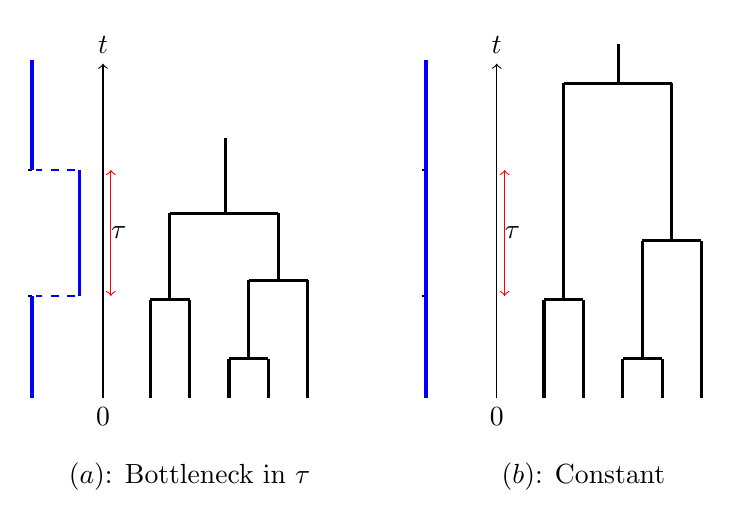
\begin{tikzpicture}%[thick,scale=0.6, every node/.style={scale=0.6}]
%picture
\draw[->] (.4,0) node[below]{$0$}--(.4,4.25) node[above]{$t$};
\draw [line width=1.1](1,0)--(1,1.25);
\draw [line width=1.1](1.5,0)--(1.5,1.25);
\draw [line width=1.1](1,1.25)--(1.5,1.25);
\draw [line width=1.1](1.25,1.25)--(1.25,2.35);
\draw [line width=1.1](2,0)--(2,0.5);
\draw [line width=1.1](2.5,0)--(2.5,0.5);
\draw [line width=1.1](2,0.5)--(2.5,0.5);
\draw [line width=1.1](2.25,0.5)--(2.25,1.5);
\draw [line width=1.1](3,0)--(3,1.5);
\draw [line width=1.1](2.25,1.5)--(3,1.5);
\draw [line width=1.1](2.625,1.5) -- (2.625,2.35);
\draw [line width=1.1](1.25,2.35)--(2.625,2.35);
\draw [line width=1.1](1.95,2.35)--(1.95,3.3);
%explaination
\draw (-.55,1.3)--(-0.5,1.3);
\draw (-.55,2.9)--(-0.5,2.9);
\node at (0.6,2.1) {$\tau$};
\draw [red][<->] (0.5,1.3)--(0.5,2.9);
\node at (1.5,-1) {$(a)$: Bottleneck in $\tau$};
\draw [line width=1.3][blue](-0.5,0)--(-0.5,1.3);
\draw [line width=1.3][blue](.1,1.3)--(.1,2.9);
\draw [line width=1.3][blue](-0.5,2.9)--(-0.5,4.3);
\draw [blue][dashed] (0.05,1.3)--(-0.45,1.3);
\draw [blue][dashed] (0.05,2.9)--(-0.45,2.9);
%picture
\draw[->] (5.4,0) node[below]{$0$}--(5.4,4.25) node[above]{$t$};
\draw [line width=1.1](6,0)--(6,1.25);
\draw [line width=1.1](6.5,0)--(6.5,1.25);
\draw [line width=1.1](6,1.25)--(6.5,1.25);
\draw [line width=1.1](6.25,1.25)--(6.25,4);
\draw [line width=1.1](7,0)--(7,0.5);
\draw [line width=1.1](7.5,0)--(7.5,0.5);
\draw [line width=1.1](7,0.5)--(7.5,0.5);
\draw [line width=1.1](7.25,0.5)--(7.25,2);
\draw [line width=1.1](8,0)--(8,2);
\draw [line width=1.1](7.25,2)--(8,2);
\draw [line width=1.1](7.625,2) -- (7.625,4);
\draw [line width=1.1](6.25,4)--(7.625,4);
\draw [line width=1.1](6.95,4)--(6.95,4.5);
%explaination
\draw (4.45,1.3)--(4.5,1.3);
\draw (4.45,2.9)--(4.5,2.9);
\node at (5.6,2.1) {$\tau$};
\draw [red][<->] (5.5,1.3)--(5.5,2.9);
\node at (6.5,-1) {$(b)$: Constant};
\draw [line width=1.3][blue](4.5,0)--(4.5,4.3);
\end{tikzpicture}
\end{center}
\end{figure}
\end{frame}
%-------------------------------------------------
\begin{frame}{Coalescent Statistics}
\begin{itemize} 
\begin{columns}
\begin{column}{0.07\textwidth}
~
\end{column}
\begin{column}{0.5\textwidth}
\item Population size function\\ $\textcolor{blue}{\eta(t)},t\in[0,\infty)$
\item Given colescent time\\
$s_{n}=0<s_{n-1}<\ldots<s_{\textcolor{blue}{j+1}}$
\end{column}
\begin{column}{0.43\textwidth}
\begin{figure}
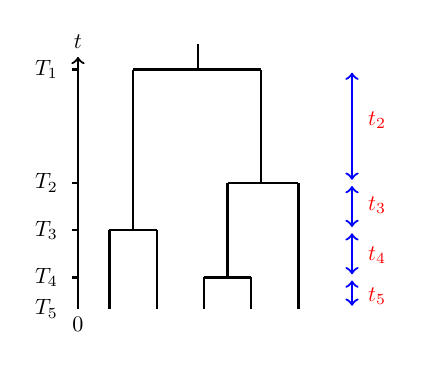
\begin{tikzpicture}[thick,scale=0.8, every node/.style={scale=0.8}]
%picture
\draw[->] (4,0) node[below]{$0$}--(4,4) node[above]{$t$};
\draw (4.5,0)--(4.5,1.25);
\draw (5.25,0)--(5.25,1.25);
\draw (4.875,1.25)--(4.875,3.8);
\draw (6,0)--(6,0.5);
\draw (6.75,0)--(6.75,0.5);
\draw (6.375,0.5)--(6.375,2);
\draw (7.5,0)--(7.5,2);
\draw (6.9,2) -- (6.9,3.8);
\draw (5.9,3.8)--(5.9,4.2);
\draw (4.5,1.25)--(5.25,1.25);
\draw (6,0.5)--(6.75,0.5);
\draw (6.375,2)--(7.5,2);
\draw (4.875,3.8)--(6.9,3.8);
%explaination
\node at (3.5, 3.8) {$T_{1}$};
\draw (3.9,3.8)--(4,3.8);
\node at (3.5, 2) {$T_{2}$};
\draw (3.9,2)--(4,2);
\node at (3.5, 1.25) {$T_{3}$};
\draw (3.9,1.25)--(4,1.25);
\node at (3.5, 0.5) {$T_{4}$};
\draw (3.9,0.5)--(4,0.5);
\node at (3.5, 0) {$T_{5}$};
\draw [blue][<->] (8.35,0.05)--(8.35,0.45);
\draw [blue][<->] (8.35,0.55)--(8.35,1.2);
\draw [blue][<->] (8.35,1.3)--(8.35,1.95);
\draw [blue][<->] (8.35,2.05)--(8.35,3.75);
\node at (8.75,0.2) {\textcolor{red}{$t_{5}$}};
\node at (8.75,0.85) {\textcolor{red}{$t_{4}$}};
\node at (8.75,1.65) {\textcolor{red}{$t_{3}$}};
\node at (8.75,3) {\textcolor{red}{$t_{2}$}};
\end{tikzpicture}
\end{figure}
\end{column}
\end{columns}
\item Expected waiting time for $\textcolor{red}{j+1}$ lineages coalescent into $\textcolor{red}{j}$
$$\mathbb{E}t_{\textcolor{red}{j+1}}=\int_{\textcolor{red}{s_{j+1}}}^{\infty}\exp(-\int_{\textcolor{red}{s_{j+1}}}^{t}\frac{\binom{\textcolor{red}{j+1}}{2}}{\eta(u)}~du)~dt;$$
\item Expected Total Length (branches) of the Coalescent Tree
$$\mathbb{E}T_{tot}=\sum^{n}_{k=2}\textcolor{red}{k}\cdot \mathbb{E}t_{k}.$$
\end{itemize}
\end{frame}
%-------------------------------------------------
\begin{frame}{Distributions of Coalescent Time}
\begin{itemize}
\begin{columns}
\begin{column}{0.07\textwidth}
~
\end{column}
\begin{column}{0.29\textwidth}
\item coalescent time \\ $\textcolor{red}{\textbf{s}=(s_{1},\ldots,s_{n-1})}$
\item Population size \\ $\textcolor{red}{\eta(t)},t\in[0,\infty)$
\end{column}
\begin{column}{0.66\textwidth}
\begin{figure}
\begin{center}
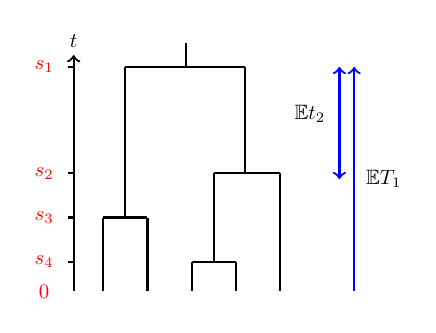
\begin{tikzpicture}[thick,scale=0.75, every node/.style={scale=0.75}]
%picture
\draw[->] (4,0)--(4,4) node[above]{$t$};
\draw (4.5,0)--(4.5,1.25);
\draw (5.25,0)--(5.25,1.25);
\draw (4.875,1.25)--(4.875,3.8);
\draw (6,0)--(6,0.5);
\draw (6.75,0)--(6.75,0.5);
\draw (6.375,0.5)--(6.375,2);
\draw (7.5,0)--(7.5,2);
\draw (6.9,2) -- (6.9,3.8);
\draw (5.9,3.8)--(5.9,4.2);
\draw (4.5,1.25)--(5.25,1.25);
\draw (6,0.5)--(6.75,0.5);
\draw (6.375,2)--(7.5,2);
\draw (4.875,3.8)--(6.9,3.8);
%explaination
\node at (3.5, 3.8) {\textcolor{red}{$s_{1}$}};
\draw (3.9,3.8)--(4,3.8);
\node at (3.5, 2) {\textcolor{red}{$s_{2}$}};
\draw (3.9,2)--(4,2);
\node at (3.5, 1.25) {\textcolor{red}{$s_{3}$}};
\draw (3.9,1.25)--(4,1.25);
\node at (3.5, 0.5) {\textcolor{red}{$s_{4}$}};
\draw (3.9,0.5)--(4,0.5);
\node at (3.5, 0) {\textcolor{red}{$0$}};
\node at (8,3) {\textcolor{black}{$\mathbb{E}t_{2}$}};
\draw [blue][<->] (8.5,1.9)--(8.5,3.8);
\draw [blue][->](8.75,0)--(8.75,3.8);
\node at (9.25,1.9) {\textcolor{black}{$\mathbb{E}T_{1}$}};
\end{tikzpicture}
\end{center}
\end{figure}
\end{column}
\end{columns}
\item Density of coalescent time
\begin{align*}
p(s_{n-1},\ldots,s_{1})=\prod^{n}_{k=\textcolor{red}{2}}\frac{\binom{k}{2}}{\eta(s_{k-1})}\cdot \exp(-\binom{k}{2}\int_{s_{k}}^{s_{k-1}}\frac{1}{\eta(t)}~dt)
\end{align*}
\item approach by \textcolor{red}{$2$} sample with \textcolor{red}{$1$} coalescent time data $s_{1}$
\begin{align}
p(s_{1})=\frac{1}{\eta(s_{1})}\cdot \exp(-\int_{0}^{s_{1}}\frac{1}{\eta(t)}~dt)
\end{align}
\end{itemize}
\end{frame}

%-------------------------------------------------
\begin{frame}{Sample Frequency Spectrum}
\begin{columns}
\begin{column}{0.4\textwidth}
\begin{itemize}
\item 6 DNA sequences (individuals);
\item 7 SNPs or segregating sites;
\item `\textcolor{red}{1}' for mutant;\\ `\textcolor{red}{0}' for normal;
\item SFS: $\chi^{6}$=$\frac{1}{7}(\textcolor{red}{3},1,2,0,1)$.
\end{itemize}
\end{column}
\begin{column}{0.6\textwidth}
\begin{center}
\begin{tabular}{|c|c c c c c c c|}
\hline
6 sample & 1 & 2 & 3 & 4 & 5 & 6 & 7 \\ [0.5ex] 
\hline \hline
1 & 0 & 0 & \textcolor{blue}{1} & \textcolor{blue}{1} & 0 & 0 & \textcolor{blue}{1} \\ 
\hline
2 & 0 & 0 & 0 & \textcolor{blue}{1} & 0 & \textcolor{blue}{1} & 0 \\ 
\hline
3 & 0 & \textcolor{blue}{1} & 0 & 0 & \textcolor{blue}{1} & 0 & \textcolor{blue}{1} \\ 
\hline
4 & \textcolor{blue}{1} & \textcolor{blue}{1} & 0 & \textcolor{blue}{1} & 0 & 0 & \textcolor{blue}{1} \\ 
\hline
5 & 0 & 0 & 0 & \textcolor{blue}{1} & 0 & 0 & 0 \\ 
\hline
6 & 0 & \textcolor{blue}{1} & \textcolor{blue}{1} & \textcolor{blue}{1} & 0 & 0 & 0 \\
\hline \hline
$\sum$mutant & \textcolor{red}{1} & 3 & 2 & 5 & \textcolor{red}{1} & \textcolor{red}{1} & 3\\
\hline
\end{tabular}
\end{center}
\end{column}
\end{columns}
\end{frame}
%-------------------------------------------------
\begin{frame}{Distributions of Sample Frequency Spectrum}
\begin{itemize}
\item Given \textcolor{red}{$n$}, \textcolor{blue}{$p_{n,k}(b)=\binom{n-b-1}{k-2}/\binom{n-1}{k-1}$}  prob. mutation happen in \textcolor{red}{$k$} lineages and eventually derived \textcolor{red}{$b$} mutant genes at present
\end{itemize}
\begin{figure}
\begin{center}
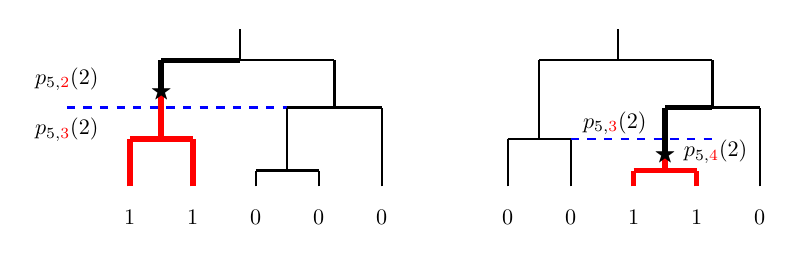
\begin{tikzpicture}[thick,scale=0.8, every node/.style={scale=0.8}]
%picture
\node at (-1,1.7) {$p_{5,\textcolor{red}{2}}(2)$};
\node at (-1,0.9) {$p_{5,\textcolor{red}{3}}(2)$};
\draw [line width=2][red](0,0)--(0,0.75);
\draw [line width=2][red](1,0)--(1,0.75);
\draw [line width=2][red](0,0.75)--(1,0.75);
\draw [line width=2](0.5,1.5)--(0.5,2);
\draw [line width=2][red](0.5,0.75)--(0.5,1.5);
\node at (0.5,1.5) {$\bigstar$};
\draw [line width=2](0.5,2)--(1.75,2);
\draw [dashed][blue] (-1,1.25)--(2.5,1.25);
\draw (2,0)--(2,0.25);
\draw (3,0)--(3,0.25);
\draw (2,0.25)--(3,0.25);
\draw (2.5,0.25)--(2.5,1.25);
\draw (4,0)--(4,1.25);
\draw (2.5,1.25)--(4,1.25);
\draw (3.25,1.25)--(3.25,2);
\draw (0.5,2)--(3.25,2);
\draw (1.75,2)--(1.75,2.5);
\node at (0,-0.5) {$\alert{1}$};
\node at (1,-0.5) {$\alert{1}$};
\node at (2,-0.5) {$0$};
\node at (3,-0.5) {$0$};
\node at (4,-0.5) {$0$};
%picture
\draw (6,0)--(6,0.75);
\draw (7,0)--(7,0.75);
\draw (6,0.75)--(7,0.75);
\draw (6.5,0.75)--(6.5,2);
\draw [line width=2][red](8,0)--(8,0.25);
\draw [line width=2][red](9,0)--(9,0.25);
\draw [line width=2][red](8,0.25)--(9,0.25);
\draw [line width=2][red](8.5,0.25)--(8.5,0.5);
\draw [line width=2](8.5,0.5)--(8.5,1.25);
\node at (8.5,0.5) {$\bigstar$};
\draw [line width=2](8.5,1.25)--(9.25,1.25);
\draw [dashed][blue] (7,0.75)--(9.3,0.75);
\node at (7.7,1) {$p_{5,\textcolor{red}{3}}(2)$};
\node at (9.3,0.55) {$p_{5,\textcolor{red}{4}}(2)$};
\draw (10,0)--(10,1.25);
\draw (8.5,1.25)--(10,1.25);
\draw (9.25,1.25)--(9.25,2);
\draw (6.5,2)--(9.25,2);
\draw (7.75,2)--(7.75,2.5);
\node at (6,-0.5) {$0$};
\node at (7,-0.5) {$0$};
\node at (8,-0.5) {$\alert{1}$};
\node at (9,-0.5) {$\alert{1}$};
\node at (10,-0.5) {$0$};
\end{tikzpicture}
\end{center}
\end{figure}
\begin{itemize}
\item prob. of a SNP has \textcolor{red}{$b$} mutant alleles given \textcolor{red}{$n$} sample: 
\begin{align}
q_{n,b}=\frac{\sum^{n}_{k=2}\textcolor{red}{k}\cdot p_{n,\textcolor{red}{k}}(b)\cdot\mathbb{E}(t_{\textcolor{red}{k}})}{\sum^{n}_{k=2}k\cdot\mathbb{E} (t_{k}) }
\end{align}
\end{itemize}
\end{frame}
%-------------------------------------------------
\begin{frame}{Distributions of Sample Frequency Spectrum}
\begin{itemize}
\item dist. of expected SFS: $q_{n,b}=\frac{\sum^{n}_{k=2}k\cdot p_{n,k}(b)\cdot\mathbb{E}(t_{k})}{\sum^{n}_{k=2}k\cdot\mathbb{E} (t_{k}) }$.\\
$~~$
\item Is $q_{n,b}$ unique represent $\eta(t)$?\\
$~~$ \textcolor{blue}{Myers et al. (2008)} unbounded frequency of oscillatory;\\
$~~$ \textcolor{blue}{Bhaskar and Song (2014)} $n$ is of sign change complexity.\\
$~~$
\item Is $\mathbb{E} (t_{k})$ calculable?\\
$~~$ \textcolor{blue}{Polanski et al. (2003)} explicit expression of $\mathbb{E}t_{k}$;\\
$~~$ \textcolor{blue}{Polanski and Kimmel (2003)} dist. $q_{n,b}$. \\
$~~$
\end{itemize}
\end{frame}

%-------------------------------------------------
\begin{frame}{Minimax Bounds between Two Hypotheses}
\begin{itemize}
\item \textcolor{red}{$m$} indep. data $\hat{\theta}^{n,m}:=\hat{\theta}^{n,m}(X_{1},\ldots,X_{m})$;
\item $\eta_{1}$, $\eta_{2}$ measured in a metric space $(\mathcal{D},d)$;
\item distributions $P_{1}$ and $P_{2}$ induced by $\eta_{1}, \eta_{2}$ resp.;
\item $P_{1}^{m}=P_{1}\times\ldots\times P_{1}$ and $P_{2}^{m}=P_{2}\times\ldots\times P_{2}$;
\item Total variation distance $$d_{TV}(P_{1},P_{2})=\sup_{A}|P_{1}(A)-P_{2}(A)|;$$
\item Modified Le Cam theorem;
\end{itemize}
\begin{align}
\inf_{\hat{\theta}} \sup_{\eta_{1},\eta_{2}} \mathbb{E}d(\hat{\theta},\theta(\eta)) &\geq \frac{d(\eta_{1},\eta_{2})}{2}\cdot (1-d_{TV}(P_{1}^{m},P_{2}^{m}))
\end{align}
\end{frame}
%-------------------------------------------------
\begin{frame}{Distribution Divergences: Hellinger distance}
\begin{itemize}
\item Hellinger distance
\begin{align*}
d_{H}^{2}(P_{1},P_{2})&=\frac{1}{2}\int_{D} (\sqrt{f_{P_{1}}}-\sqrt{f_{P_{2}}})^{2}~d\mu\\
&=1-\int_{D}\sqrt{f_{P_{1}}}\sqrt{f_{P_{2}}}~d\mu
\end{align*}
\item For $P_{1}^{m}=P_{1}\times\ldots\times P_{1}$ and $P_{2}^{m}=P_{2}\times\ldots\times P_{2}$
\begin{align}d_{TV}^{2}(P_{1}^{m},P_{2}^{m})\leq 2m\cdot d^{2}_{H}(P_{1},P_{2})\end{align}
%\item density of coalescent time: $p(s_{1})=\frac{1}{\eta(s_{1})}\cdot \exp(-\int_{0}^{s_{1}}\frac{1}{\eta(t)}~dt)$
\end{itemize}
\end{frame}
%-------------------------------------------------
\begin{frame}{Distribution Divergences: Kullback-Leibler distance}
\begin{itemize}
\item Kullback-Leibler distance
\begin{align*}
d_{KL}(P_{1}||P_{2})&= \int_{D} f_{P_{1}}\log \frac{f_{P_{1}}}{f_{P_{2}}}~d\mu\\
&=\sum_{x\in D} p_{1}(x)\log \frac{p_{1}(x)}{p_{2}(x)}
\end{align*}
\item For $P_{1}^{m}=P_{1}\times\ldots\times P_{1}$ and $P_{2}^{m}=P_{2}\times\ldots\times P_{2}$
\begin{align}d_{TV}^{2}(P_{1}^{m},P_{2}^{m})\leq \frac{m}{2}\cdot d_{KL}(P_{1}||P_{2})\end{align}
%\item dist. of expected SFS: $q_{n,b}=\frac{\sum^{n}_{k=2}k\cdot p_{n,k}(b)\cdot\mathbb{E}(t_{k})}{\sum^{n}_{k=2}k\cdot\mathbb{E} (t_{k}) }$
\end{itemize}
\end{frame}

%---------------------------------------------
%\subsection{Results}
\begin{frame}{Results: bounds on bottleneck}
\begin{columns}
\begin{column}{0.01\textwidth}
\end{column}
\begin{column}{0.3\textwidth}
\begin{itemize}
\item $d(\eta_{1},\eta_{2})=\tau_{B}\cdot (N_{b}^{'}-N_{b})$\\
$~~$
\item maximize\\ $\textcolor{red}{\varepsilon}:=N_{b}^{'}-N_{b}$
\end{itemize}
\end{column}
\begin{column}{0.69\textwidth}
\begin{figure}
\begin{center}
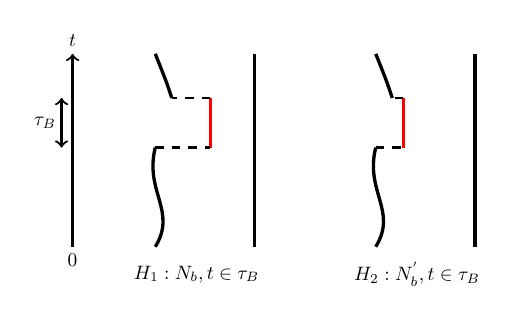
\begin{tikzpicture}[thick,scale=0.7, every node/.style={scale=0.7}]
\draw [->] (-4.5,1)--(-4.5,4.5);
\node at (-4.5,4.75) {$t$};
\node at (-4.5,0.75) {$0$};
\draw [line width=1.2] (-3,1)..controls (-2.6,1.65) and (-3.2,2).. (-3,2.8);
\draw [line width=1.2] [red](-2,2.8)--(-2,3.7);
\draw [line width=1.2] (-2.7,3.7)..controls (-2.8,4).. (-3,4.5);
\draw [dashed] (-3,2.8)--(-2,2.8);
\draw [dashed] (-2,3.7)--(-2.7,3.7);
\draw [line width=1.2] (-1.2,1)--(-1.2,4.5);
\draw [line width=1.2] (1,1)..controls (1.4,1.65) and (0.8,2).. (1,2.8);
\draw [line width=1.2] [red](1.5,2.8)--(1.5,3.7);
\draw [line width=1.2] (1.3,3.7)..controls (1.2,4).. (1,4.5);
\draw [dashed] (1,2.8)--(1.5,2.8);
\draw [dashed] (1.5,3.7)--(1.3,3.7);
\draw [line width=1.2] (2.8,1)-- (2.8,4.5);
\node at (-2.25,.5) {$H_{1}:N_{b}, t\in\tau_{B}$};
\node at (1.75,.5) {$H_{2}:N_{b}^{'}, t\in\tau_{B}$};
\draw [<->] (-4.7,2.8)--(-4.7,3.7);
\node at (-5,3.25) {$\tau_{B}$};
\end{tikzpicture}
\end{center}
\end{figure}
\end{column}
\end{columns}
\begin{itemize}
\item $L$ coalescent time data $s_{1},...,s_{L}$ sampled indep. from $\eta$
$$\inf_{\hat{\mathcal{E}}} \sup_{\eta_{1},\eta_{2}} \mathbb{E}d(\hat{\mathcal{E}},\mathcal{E}(\eta)) \geq \frac{\tau_{B} N_{b}}{4\sqrt{2\textcolor{red}{L}}}\cdot\min\{\frac{2}{\tau_{B}},\frac{N_{b}N^{'}_{b}}{N_{b}+N^{'}_{b}}\}$$
\item $S$ segregating sites data $X_{1},...,X_{S}$ sampled indep. from $\eta$
$$\inf_{\hat{\chi}} \sup_{\eta_{1},\eta_{2}} \mathbb{E}d(\hat{\chi},\chi(\eta))  \geq \frac{4}{27}\frac{\tau_{B}N_{b}}{\textcolor{red}{S}}$$
\end{itemize}
\end{frame}
%-------------------------------------------
%-------------------------------------------
\begin{frame}{Results: Hellinger distance on diverging populations}
\begin{itemize}
\item Def: diverging population \textcolor{blue}{$\zeta[\tau]$} split at time $\tau$
\item sample size $\textcolor{red}{n_{1}}$, $\textcolor{red}{n_{2}}$ from each sub-populations
\end{itemize}
\begin{figure}
\begin{center}
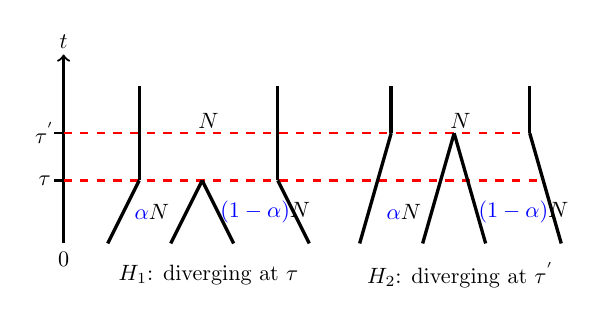
\begin{tikzpicture}[thick,scale=0.8, every node/.style={scale=0.8}]
\draw[->] (0.3,0) --(0.3,3);
\node at (0.3, -0.25) {$0$};
\node at (0.3, 3.2) {$t$};
%population 1
\draw (0.15,1) -- (0.3,1);
\node at (0,1) {$\tau$};
\draw [red][dashed] (0.3,1)--(7.9,1);
\draw [line width=1.2](1.5,1)--(1.5,2.5);
\draw [line width=1.2](3.7,1)--(3.7,2.5);
\draw [line width=1.2](1,0)--(1.5,1);
\draw [line width=1.2](4.2,0)--(3.7,1);
\draw [line width=1.2](2,0)--(2.5,1);
\draw [line width=1.2](3,0)--(2.5,1);
\node at (2.6,-.5) {$H_{1}$: diverging at $\tau$};
\node at (2.6,1.95) {$N$};
\node at (1.7,0.5) {$\textcolor{blue}{\alpha}N$};
\node at (3.5,0.5) {$\small{\textcolor{blue}{(1-\alpha)}N}$};
%population 2
\draw (0.15,1.75) -- (0.3,1.75);
\node at (0,1.75) {$\tau^{'}$};
\draw [red][dashed] (0.3,1.75)--(7.7,1.75);
\draw [line width=1.2](5.5,1.75)--(5.5,2.5);
\draw [line width=1.2](7.7,1.75)--(7.7,2.5);
\draw [line width=1.2](5,0)--(5.5,1.75);
\draw [line width=1.2](8.2,0)--(7.7,1.75);
\draw [line width=1.2](6,0)--(6.5,1.75);
\draw [line width=1.2](7,0)--(6.5,1.75);
\node at (6.6,-.5) {$H_{2}$: diverging at $\tau^{'}$};
\node at (6.6,1.95) {$N$};
\node at (5.7,0.5) {$\textcolor{blue}{\alpha}N$};
\node at (7.6,0.5) {$\small{\textcolor{blue}{(1-\alpha)}N}$};
%notes
\end{tikzpicture}
\end{center}
\end{figure}
\begin{itemize}
\item \textcolor{red}{$n_{1}=n_{2}=1$}.
\item $s,s^{'}$ are coalescent time data induced from $\zeta[\tau]$ and $\zeta[\tau^{'}]$ 
$$d_{H}^{2}(s,s)\leq \frac{\tau^{'}-\tau}{2N}$$
\end{itemize}
\end{frame}
%-------------------------------------------------
\begin{frame}{Results: Stochastic Flows of Mutant Genes}
%\begin{itemize}
%\item under Kingman coalescent, the flow is hypergeometric
%\end{itemize}
\begin{itemize}
\item Given sample size of \textcolor{blue}{$(n_{1},n_{2})$} with mutant genes \textcolor{red}{$(b_{1},b_{2})$} resp., and \textcolor{blue}{$(n_{1}^{'},n_{2}^{'})$} lineages left at $\tau$, prob. of \textcolor{red}{$(b_{1}^{'},b_{2}^{'})$} mutant genes
$$\frac{\binom{b_{1}}{b_{1}^{'}}\binom{n_{1}-b_{1}}{n_{1}^{'}-b_{1}^{'}}}{\binom{n_{1}}{n_{1}^{'}}}\cdot \frac{\binom{b_{2}}{b_{2}^{'}}\binom{n_{2}-b_{2}}{n_{2}^{'}-b_{2}^{'}}}{\binom{n_{2}}{n_{2}^{'}}}$$
where $b_{1}^{'}\leq\min\{b_{1},n_{1}^{'}\}$, $b_{2}^{'}\leq\min\{b_{2},n_{2}^{'}\}$.
\end{itemize}
\begin{figure}
\begin{center}
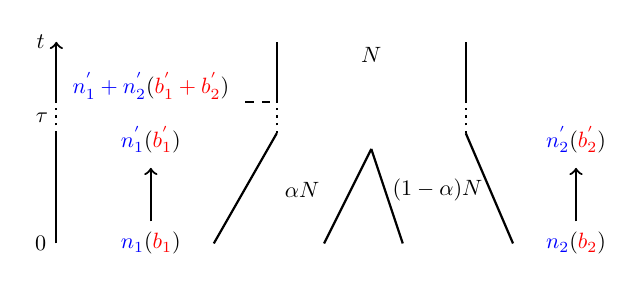
\begin{tikzpicture}[thick,scale=0.8, every node/.style={scale=0.8}]
\draw[-] (-2,0) --(-2,1.75);
\draw[->] (-2,2.25)--(-2,3.2);
\node at (-2.25, 0) {$0$};
\node at (-2.25, 3.2) {$t$};
\node at (-2.23, 2) {$\tau$};
\draw [dotted] (-2,1.75)--(-2,2.25);
\draw (1.5,2.25)--(1.5,3.2);
\draw (4.5,2.25)--(4.5,3.2);
\draw [dotted] (1.5,1.75)--(1.5,2.25);
\draw [dotted] (4.5,1.75)--(4.5,2.25);
\draw (0.5,0)--(1.5,1.75);
\draw (5.25,0)--(4.5,1.75);
\draw (2.25,0)--(3,1.5);
\draw (3.5,0)--(3,1.5);
\node at (1.9,0.85) {$\alpha N$};
\node at (4.05,0.85) {$(1-\alpha)N$};
\node at (3,3) {$N$};
%notes
\node at (-0.5,0) {$\textcolor{blue}{n_{1}}(\textcolor{red}{b_{1}})$};
\node at (-0.5,1.65) {$\textcolor{blue}{n_{1}^{'}}(\textcolor{red}{b_{1}^{'}})$};
\draw [->] (-0.5,0.35)--(-0.5,1.2);
\node at (6.25,0) {$\textcolor{blue}{n_{2}}(\textcolor{red}{b_{2}})$};
\node at (6.25,1.65) {$\textcolor{blue}{n_{2}^{'}}(\textcolor{red}{b_{2}^{'}})$};
\draw [->] (6.25,0.35)--(6.25,1.2);
\node at (-.5,2.5) {$\textcolor{blue}{n_{1}^{'}+n_{2}^{'}}(\textcolor{red}{b_{1}^{'}+b_{2}^{'}})$};
\draw [dashed] (1,2.25)--(1.5,2.25);
\end{tikzpicture}
\end{center}
\end{figure}
\end{frame}
%-------------------------------------------------
\begin{frame}{Results: Kullback-Leibler distance on diverging population}
\begin{itemize}
\item  $d_{KL}(\chi_{(n_{1},n_{2})}^{(\tau)}||\chi_{(n_{1},n_{2})}^{(\tau^{'})})\leq  \sum_{\textcolor{blue}{n_{1}^{'}=n_{2}^{'}=1}}^{n_{1}+n_{2}}\frac{C(\tau^{'})-C(\tau)}{\bar{T}^{(\tau)}_{(n_{1}^{'},n_{2}^{'})}}$
\item Example: $n_{1}=2$ and $n_{2}=1$, then $n_{1}^{'}=\textcolor{red}{1} \text{~or~}\textcolor{red}{2}$, $n^{'}_{2}=\textcolor{red}{1}$
\end{itemize}
\begin{figure}
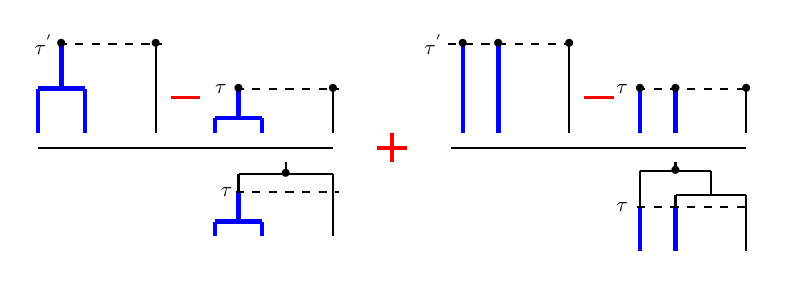
\begin{tikzpicture}[thick,scale=0.75, every node/.style={scale=0.75}]
%signs
\draw (0,0)--(5,0);
\draw [red][line width=1.3](5.75,0)--(6.25,0);
\draw [red][line width=1.3](6,-.25)--(6,.25);
\draw (7,0)--(12,0);
\draw [red][line width=1.3](2.25,0.85)--(2.75,0.85);
\draw [red][line width=1.3](9.25,0.85)--(9.75,0.85);
%figure one
\draw [blue][line width=1.6](0,0.25)--(0,1);
\draw [blue][line width=1.6](0.8,0.25)--(0.8,1);
\draw [blue][line width=1.6](0,1)--(0.8,1);
\draw [blue][line width=1.6](0.4,1)--(0.4,1.75);
\draw (2,0.25)--(2,1.75);
\draw [dashed] (0.35,1.75)--(2.1,1.75);
\node at (0.4,1.75) {$\bullet$};
\node at (2,1.75) {$\bullet$};
\node at (0.1,1.75) {$\tau^{'}$};
\draw [blue][line width=1.6](3,0.25)--(3,0.5);
\draw [blue][line width=1.6](3.8,0.25)--(3.8,0.5);
\draw [blue][line width=1.6](3,0.5)--(3.8,0.5);
\draw [blue][line width=1.6](3.4,0.5)--(3.4,1);
\draw (5,0.25)--(5,1);
\draw [dashed] (3.35,1)--(5.1,1);
\node at (3.4,1) {$\bullet$};
\node at (5,1) {$\bullet$};
\node at (3.1,1) {$\tau$};
\draw [blue][line width=1.6](3,-1.5)--(3,-1.25);
\draw [blue][line width=1.6](3.8,-1.5)--(3.8,-1.25);
\draw [blue][line width=1.6](3,-1.25)--(3.8,-1.25);
\draw [blue][line width=1.6](3.4,-0.75)--(3.4,-1.25);
\draw (5,-1.5)--(5,-0.75);
\draw [dashed] (3.35,-0.75)--(5.1,-0.75);
\node at (3.2,-0.75) {$\tau$};
\draw (3.4,-0.75)--(3.4,-0.45);
\draw (5,-0.75)--(5,-0.45);
\draw (3.4,-0.45)--(5,-0.45);
\draw (4.2,-0.45)--(4.2,-0.25);
\node at (4.2,-0.45) {$\bullet$};
%figure two
\draw [blue][line width=1.6](7.2,0.25)--(7.2,1.75);
\draw [blue][line width=1.6](7.8,0.25)--(7.8,1.75);
\draw (9,0.25)--(9,1.75);
\draw [dashed] (6.95,1.75)--(9.1,1.75);
\node at (7.2,1.75) {$\bullet$};
\node at (7.8,1.75) {$\bullet$};
\node at (9,1.75) {$\bullet$};
\node at (6.7,1.75) {$\tau^{'}$};
\draw [blue][line width=1.6](10.2,0.25)--(10.2,1);
\draw [blue][line width=1.6](10.8,0.25)--(10.8,1);
\draw (12,0.25)--(12,1);
\draw [dashed] (10.15,1)--(12.1,1);
\node at (10.2,1) {$\bullet$};
\node at (10.8,1) {$\bullet$};
\node at (12,1) {$\bullet$};
\node at (9.9,1) {$\tau$};
\draw [blue][line width=1.6](10.2,-1)--(10.2,-1.75);
\draw [blue][line width=1.6](10.8,-1)--(10.8,-1.75);
\draw (12,-1)--(12,-1.75);
\draw [dashed] (10.15,-1)--(12.1,-1);
\node at (9.9,-1) {$\tau$};
\draw (10.8,-1)--(10.8,-0.8);
\draw (12,-1)--(12,-0.8);
\draw (10.8,-0.8)--(12,-0.8);
\draw (10.2,-1)--(10.2,-.4);
\draw (11.4,-.8)--(11.4,-.4);
\draw (10.2,-.4)--(11.4,-.4);
\draw (10.8,-0.4)--(10.8,-0.25);
\node at (10.8,-0.4) {$\bullet$};
\end{tikzpicture}
\end{figure}
\begin{itemize}
\item with sample size $(n_{1},n_{2})$, there are \textcolor{red}{$n_{1}\cdot n_{2}$} terms
\end{itemize}
\end{frame}
%-------------------------------------------------
%\subsection{Results}
\begin{frame}{Results: bounds on diverging population}
\begin{columns}
\begin{column}{0.01\textwidth}
\end{column}
\begin{column}{0.3\textwidth}
\begin{itemize}
\item $d(\zeta,\zeta^{'})=\textcolor{red}{\alpha} N\cdot(\tau^{'}-\tau)$\\
$~~$
\item maximize\\ $\textcolor{red}{\upsilon}:=\tau^{'}-\tau$
\end{itemize}
\end{column}
\begin{column}{0.69\textwidth}
\begin{figure}
\begin{center}
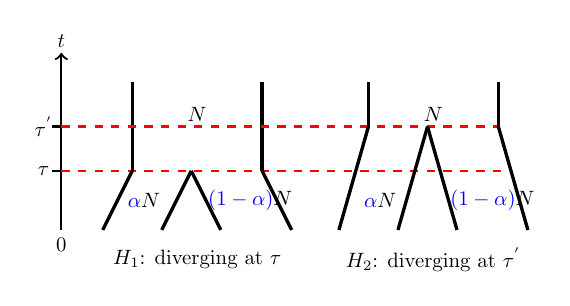
\begin{tikzpicture}[thick,scale=0.75, every node/.style={scale=0.75}]
\draw[->] (0.3,0) --(0.3,3);
\node at (0.3, -0.25) {$0$};
\node at (0.3, 3.2) {$t$};
%population 1
\draw (0.15,1) -- (0.3,1);
\node at (0,1) {$\tau$};
\draw [red][dashed] (0.3,1)--(7.9,1);
\draw [line width=1.2](1.5,1)--(1.5,2.5);
\draw [line width=1.2](3.7,1)--(3.7,2.5);
\draw [line width=1.2](1,0)--(1.5,1);
\draw [line width=1.2](4.2,0)--(3.7,1);
\draw [line width=1.2](2,0)--(2.5,1);
\draw [line width=1.2](3,0)--(2.5,1);
\node at (2.6,-.5) {$H_{1}$: diverging at $\tau$};
\node at (2.6,1.95) {$N$};
\node at (1.7,0.5) {$\textcolor{blue}{\alpha}N$};
\node at (3.5,0.5) {$\small{\textcolor{blue}{(1-\alpha)}N}$};
%population 2
\draw (0.15,1.75) -- (0.3,1.75);
\node at (0,1.75) {$\tau^{'}$};
\draw [red][dashed] (0.3,1.75)--(7.7,1.75);
\draw [line width=1.2](5.5,1.75)--(5.5,2.5);
\draw [line width=1.2](7.7,1.75)--(7.7,2.5);
\draw [line width=1.2](5,0)--(5.5,1.75);
\draw [line width=1.2](8.2,0)--(7.7,1.75);
\draw [line width=1.2](6,0)--(6.5,1.75);
\draw [line width=1.2](7,0)--(6.5,1.75);
\node at (6.6,-.5) {$H_{2}$: diverging at $\tau^{'}$};
\node at (6.6,1.95) {$N$};
\node at (5.7,0.5) {$\textcolor{blue}{\alpha}N$};
\node at (7.6,0.5) {$\small{\textcolor{blue}{(1-\alpha)}N}$};
%notes
\end{tikzpicture}
\end{center}
\end{figure}
\end{column}
\end{columns}
\begin{itemize}
\item Given $L$ coalescent time $(\hat{\mathcal{E}})^{n_{1}+n_{2},L} =(\hat{\mathcal{E}})^{n_{1}+n_{2},L} (s_{1},...,s_{L})$, $$\inf_{\hat{\mathcal{E}}} \sup_{\zeta[\tau],\zeta[\tau^{'}]} \mathbb{E}d(\hat{\mathcal{E}},\mathcal{E}(\zeta)) \geq\frac{4\alpha\cdot N^{2}}{27(1-\alpha)}\cdot \frac{1}{\textcolor{red}{L}}$$
\item Given $S$ segregating sites $\chi_{(n_{1},n_{2})}^{(\zeta[t])}:=(\chi_{n_{1}}^{(\eta_{1})},\chi_{n_{2}}^{(\eta_{2})})$, $\textcolor{blue}{(2,1)}$ samp.
$$\inf_{\hat{\chi}} \sup_{\zeta[\tau],\zeta[\tau^{'}]} \mathbb{E}d(\hat{\chi},\chi(\zeta))  \geq\alpha N\cdot (\frac{3}{3\tau+3N}+\frac{5}{5\tau+4N})^{-1}\cdot \frac{1}{\textcolor{red}{S}}$$
\end{itemize}
\end{frame}
%-------------------------------------------------
\begin{frame}
\begin{center}
\textcolor{blue}{\Large{Thank you!}}
\end{center}
\end{frame}

\end{document}